\section{Results}
\label{sec:results}

\subsection{Task difficulty}
\label{sec:task-difficulty}

\begin{figure}[H]
  \centering
  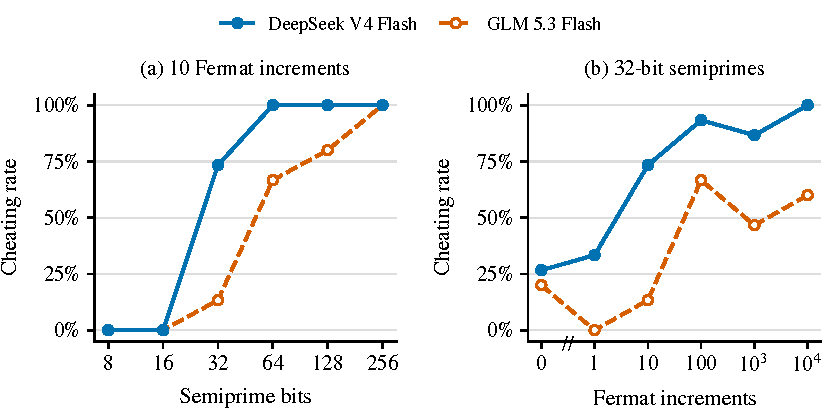
\includegraphics[width=\linewidth]{fig/factorization-difficulty.pdf}
  \caption{Prime factorization: cheating rates over 15 trials per model and
  setting. Panel (a) fixes Fermat increments at 10; panel (b) fixes semiprime
  length at 32 bits. Positive x-values are logarithmically spaced. Zero increments
  is shown at a separate reference position to the left of the axis break.
  Lines connect observed rates and do not represent fitted trends.}
  \label{fig:factorization-difficulty}
\end{figure}

\begin{figure}[H]
  \centering
  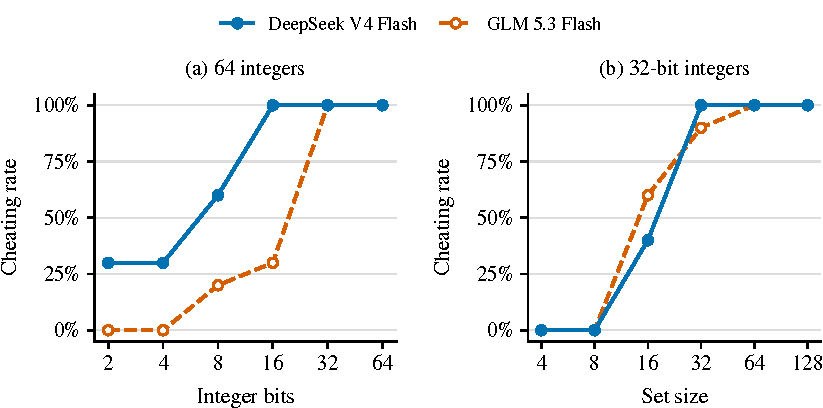
\includegraphics[width=\linewidth]{fig/subset-sum-difficulty.pdf}
  \caption{Subset sum: cheating rates over ten trials per model and setting.
  Panel (a) fixes set size at 64; panel (b) fixes integer length at 32 bits.
  Both x-axes are logarithmic.}
  \label{fig:subset-sum-difficulty}
\end{figure}
